\section{DATABASE STRUCTURE DESIGN}
\label{section:design}

\subsection{Overview of Database}
\label{sect:sub-title}
Four main entities involved in our database are Customer, Product, Order and Address. The database store necessary information about entities and their relationships. 
And the entity Schema include \par
• Customer \{Customer ID, Customer Name, Segment\}\par
• Product \{Product ID, Category, Sub-Category, Product Name\}\par
• Order \{Order ID, Customer ID, Product ID, Order Date, Ship Date, Ship Mode, Sales, Quantity, Discount, Profit, Postal Code\}\par
• Address \{Postal Code, Country, City, State, Region\}\par
And the meaning of each attribute is as following: \par
• Order ID => Unique Order ID for each Customer. \par
• Order Date => Order Date of the product. \par
• Ship Date => Shipping Date of the Product. \par
• Ship Mode=> Shipping Mode specified by the Customer. \par
• Customer ID => Unique ID to identify each Customer. \par
• Customer Name => Name of the Customer. \par
• Segment => The segment where the Customer belongs. \par
• Country => Country of residence of the Customer. \par
• City => City of residence of of the Customer. \par
• State => State of residence of the Customer. \par
• Postal Code => Postal Code of every Customer. \par
• Region => Region where the Customer belong. \par
• Product ID => Unique ID of the Product. \par 
• Category => Category of the product ordered. \par
• Sub-Category => Sub-Category of the product ordered. \par
• Product Name => Name of the Product. \par
• Sales => Sales of the Product. \par
• Quantity => Quantity of the Product. \par
• Discount => Discount provided. \par
• Profit => Profit/Loss incurred. \par
Order is a weak entity, whose existence is dependent on Customer and Product. It is because that customers have to buy products to form orders. The combination of Order ID, Customer ID and Product ID determines the unique order transaction. \par
Customer have a many-to-many relationship with Address, and every customer should have at least one address. This is because a customer must have at least one delivery address to make an order, and a customer can have multiple delivery addresses, while multiple customers can have the same delivery address.

\subsection{E-R Diagram}
\label{sect:sub-title}
The ER-Diagram(Fig.1) of our system contains four entities and two relations.
\begin{figure}[H]
    \centering
    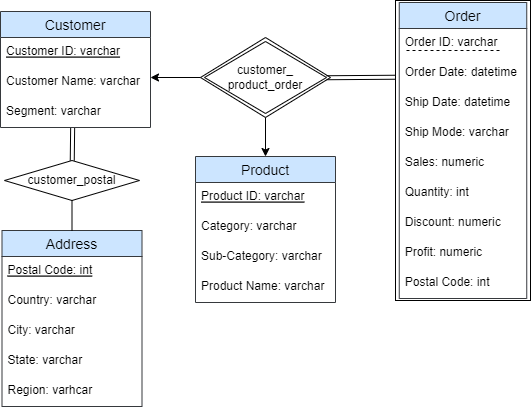
\includegraphics[width=\columnwidth]{images/ER.png}
    \caption[Short text]{ER Diagram of Supermarket Management System.}
    \label{fig:ER}
\end{figure}

\subsection{Relational Schema}
\label{sect:sub-title}
The relational schema generated from gieven ER diagram is as following: \par
• Customer \{\underline{CustomerID}, CustomerName, Segment\} \par
• Product \{\underline{ProductID}, Category, SubCategory, ProductName\}  \par
• Order \{\underline{OrderID}, \underline{CustomerID}, \underline{ProductID}, OrderDate, ShipDate, ShipMode, Sales, Quantity, Discount, Profit, PostalCode\} \par
• Address \{\underline{PostalCode}, segment, Country, City, State, Region\} \par
• customer\_postal \{\underline{CustomerID}, \underline{PostalCode}\}\par
$Customer$ contains the information of the customer except the address. $Product$ contains the information of the product. $Order$ contains the information of the order. $Address$ contains all possible address information of all customers. $customer\_postal$ contains the many to many relationship between $Customer$ and $Address$.

\subsection{Foreign key Constraint}
\label{sect:sub-title}
The forerign key referencing in our schema is as following:\par
• $CustomerID$ in $Order$ is a foreign key from $Order$ referencing $Customer$. 
Explaination: $Order$ and $Customer$ are linked through $CustomerID$. In this way, we can refer to the customer who made the specific order. An order 
cannot exist without a customer. \par
• $ProductID$ in $Order$ is a foreign key from $Order$ referencing $Customer$. 
Explaination: $Order$ and $Product$ are linked through $ProductID$. In this way, we can refer to the product which was purchased in the specific order. An order cannot exist without a purchased product. \par
• $PostalCode$ in $Order$ is a foreign key from $Order$ referencing $Address$. 
Explaination: In this way, we can check the constraint that the combination of $CustomerID$ and $PostalCode$ should exist in $customer\_postal$. If not, we can reject the order, and ask whether the customer would like to update his or her address. \par
• $CustomerID$ in $customer\_postal$ is a foreign key from $customer\_postal$ referencing $Customer$. And $PostalCode$ in $customer\_postal$ is a foreign key from $customer\_postal$ referencing $Address$. 
Explaination: $Customer$ and $Address$ are linked through  $customer\_postal$. In this way, we can refer to the 
address of a specific customer, and refer to the customer of a specific address, while saving a lot of memory. \par

\subsection{Functional Dependency}
\label{sect:sub-title}
The functional dependencies in our schema are as following:\par
• CustomerID → CustomerName, Segment \par
• ProductID → Category, SubCategory, ProductName\par
• \{OrderID, CustomerID, ProductID\} →  OrderDate, ShipDate, ShipMode, Sales, Quantity, Discount, Profit, PostalCode\par
• PostalCode → Country, City, State, Region \par

\subsection{Normalization of Schema}
\label{sect:sub-title}
Since its domain is atomic, no partial dependency, no transitive dependency, so it meets Boyce-Codd normal form, so it meets Boyce-Codd normal form (BCNF). However, considering that in some datasets, the product name may become the candidate key (in our dataset, the product name is not the candidate key), we tend to declare third normal form (3NF) here.

\subsection{Index and Hashing}
\label{sect:sub-title}
\paragraph{CustomerID}
In our dataset, $CustomerID$ contains some information about $CustormerName$: The combination of the first letter of the $CustormerName$ is the prefix of the $custormerID$. E.g. CG-12520 for Claire Gute. \par
In this way, when searching for customers with a specific customer name, non-target objects can be quickly filtered out by the two-letter prefix of CustomerID.

\paragraph{ProductID}
$ProductID$ contains some information about $Category$ and $SubCategory$: The combination of the shortcut of the $Category$ and $SubCategory$ is the prefix of the $ProductID$. E.g. FUR-BO-10001798 for Category of Furniture, and Sub-Category of Bookcases. \par
In this way, when searching for products with a specific Category and Sub-Category, non-target objects can be quickly filtered out by the “3+2”-letter prefix of ProductID. 
\\
\\
In our data, every transaction can be located using {OrderID, CustomerID, ProductID}, and those attributes are consist of Alphabetical prefixes and numeric suffixes, we can hash based on its letter prefix to speed up the search.
